%!TEX root = main.tex
\section{Resultados experimentales}

A la espera de resultados experimentales.


\begin{figure}[!t]
    \centering
    \begin{minipage}{0.9\linewidth}
    {\footnotesize
    \begin{lstlisting}[language=TeX]
\documentclass[twocolumn,twoside]{Jornadas}  

\begin{document} 
    
\title{Usando la hoja de estilo ...} 
    
\author{Uno \thanks{Una Univ.}
        y Otro \thanks{Otra Univ.}} 
\maketitle
\markboth{}{}
\pagestyle{empty} 
\thispagestyle{empty}
    
\begin{abstract} 
Este artículo ... 
\end{abstract} 
    
\begin{keywords} 
Hoja de estilo, ... 
\end{keywords} 
    
\section{Introducción} 
\PARstart{L}{a} hoja de estilo ... 
    
\begin{table}[htb] 
\caption{Ejemplo de tabla...} 
\begin{center}{\tt 
    \begin{tabular} 
    ... 
    \end{tabular}} 
\end{center} 
\end{table} 
... 
\begin{figure}[htb] 
\begin{center} 
    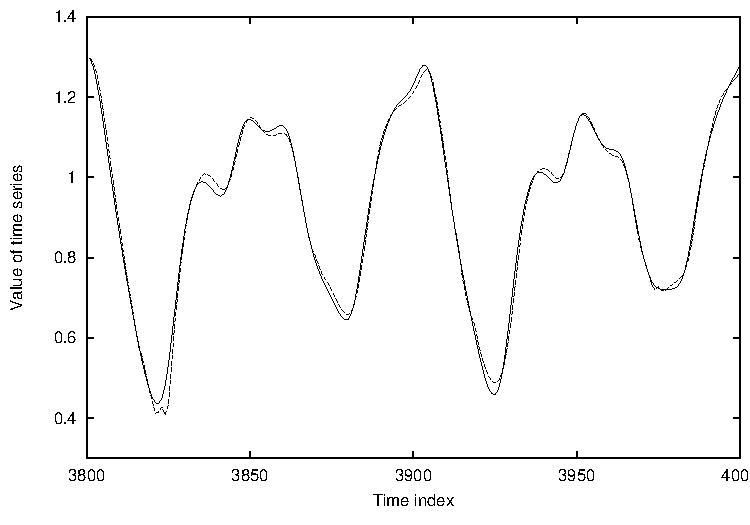
\includegraphics[width=7.5cm]{figura.pdf} 
\end{center} 
\caption{Comparación de la serie ...} 
\label{fig:curva}\end{figure} 
... 

\bibliographystyle{Jornadas} 
\bibliography{fichero.bib} 
\end{document} 
    \end{lstlisting}
    }
    \end{minipage}
    \caption{Entrada para producir este artículo. Este comentario a la figura 
    va al final de la definición de la figura.}
    \label{fig:programa}
    \end{figure}